
\begin{enumerate}
\item 
\question{Draw the circuit in Figure~\ref{figLogicGateExample} yourself.  Identify the function of each resistor.}
\solution{
The circuit is repeated below:
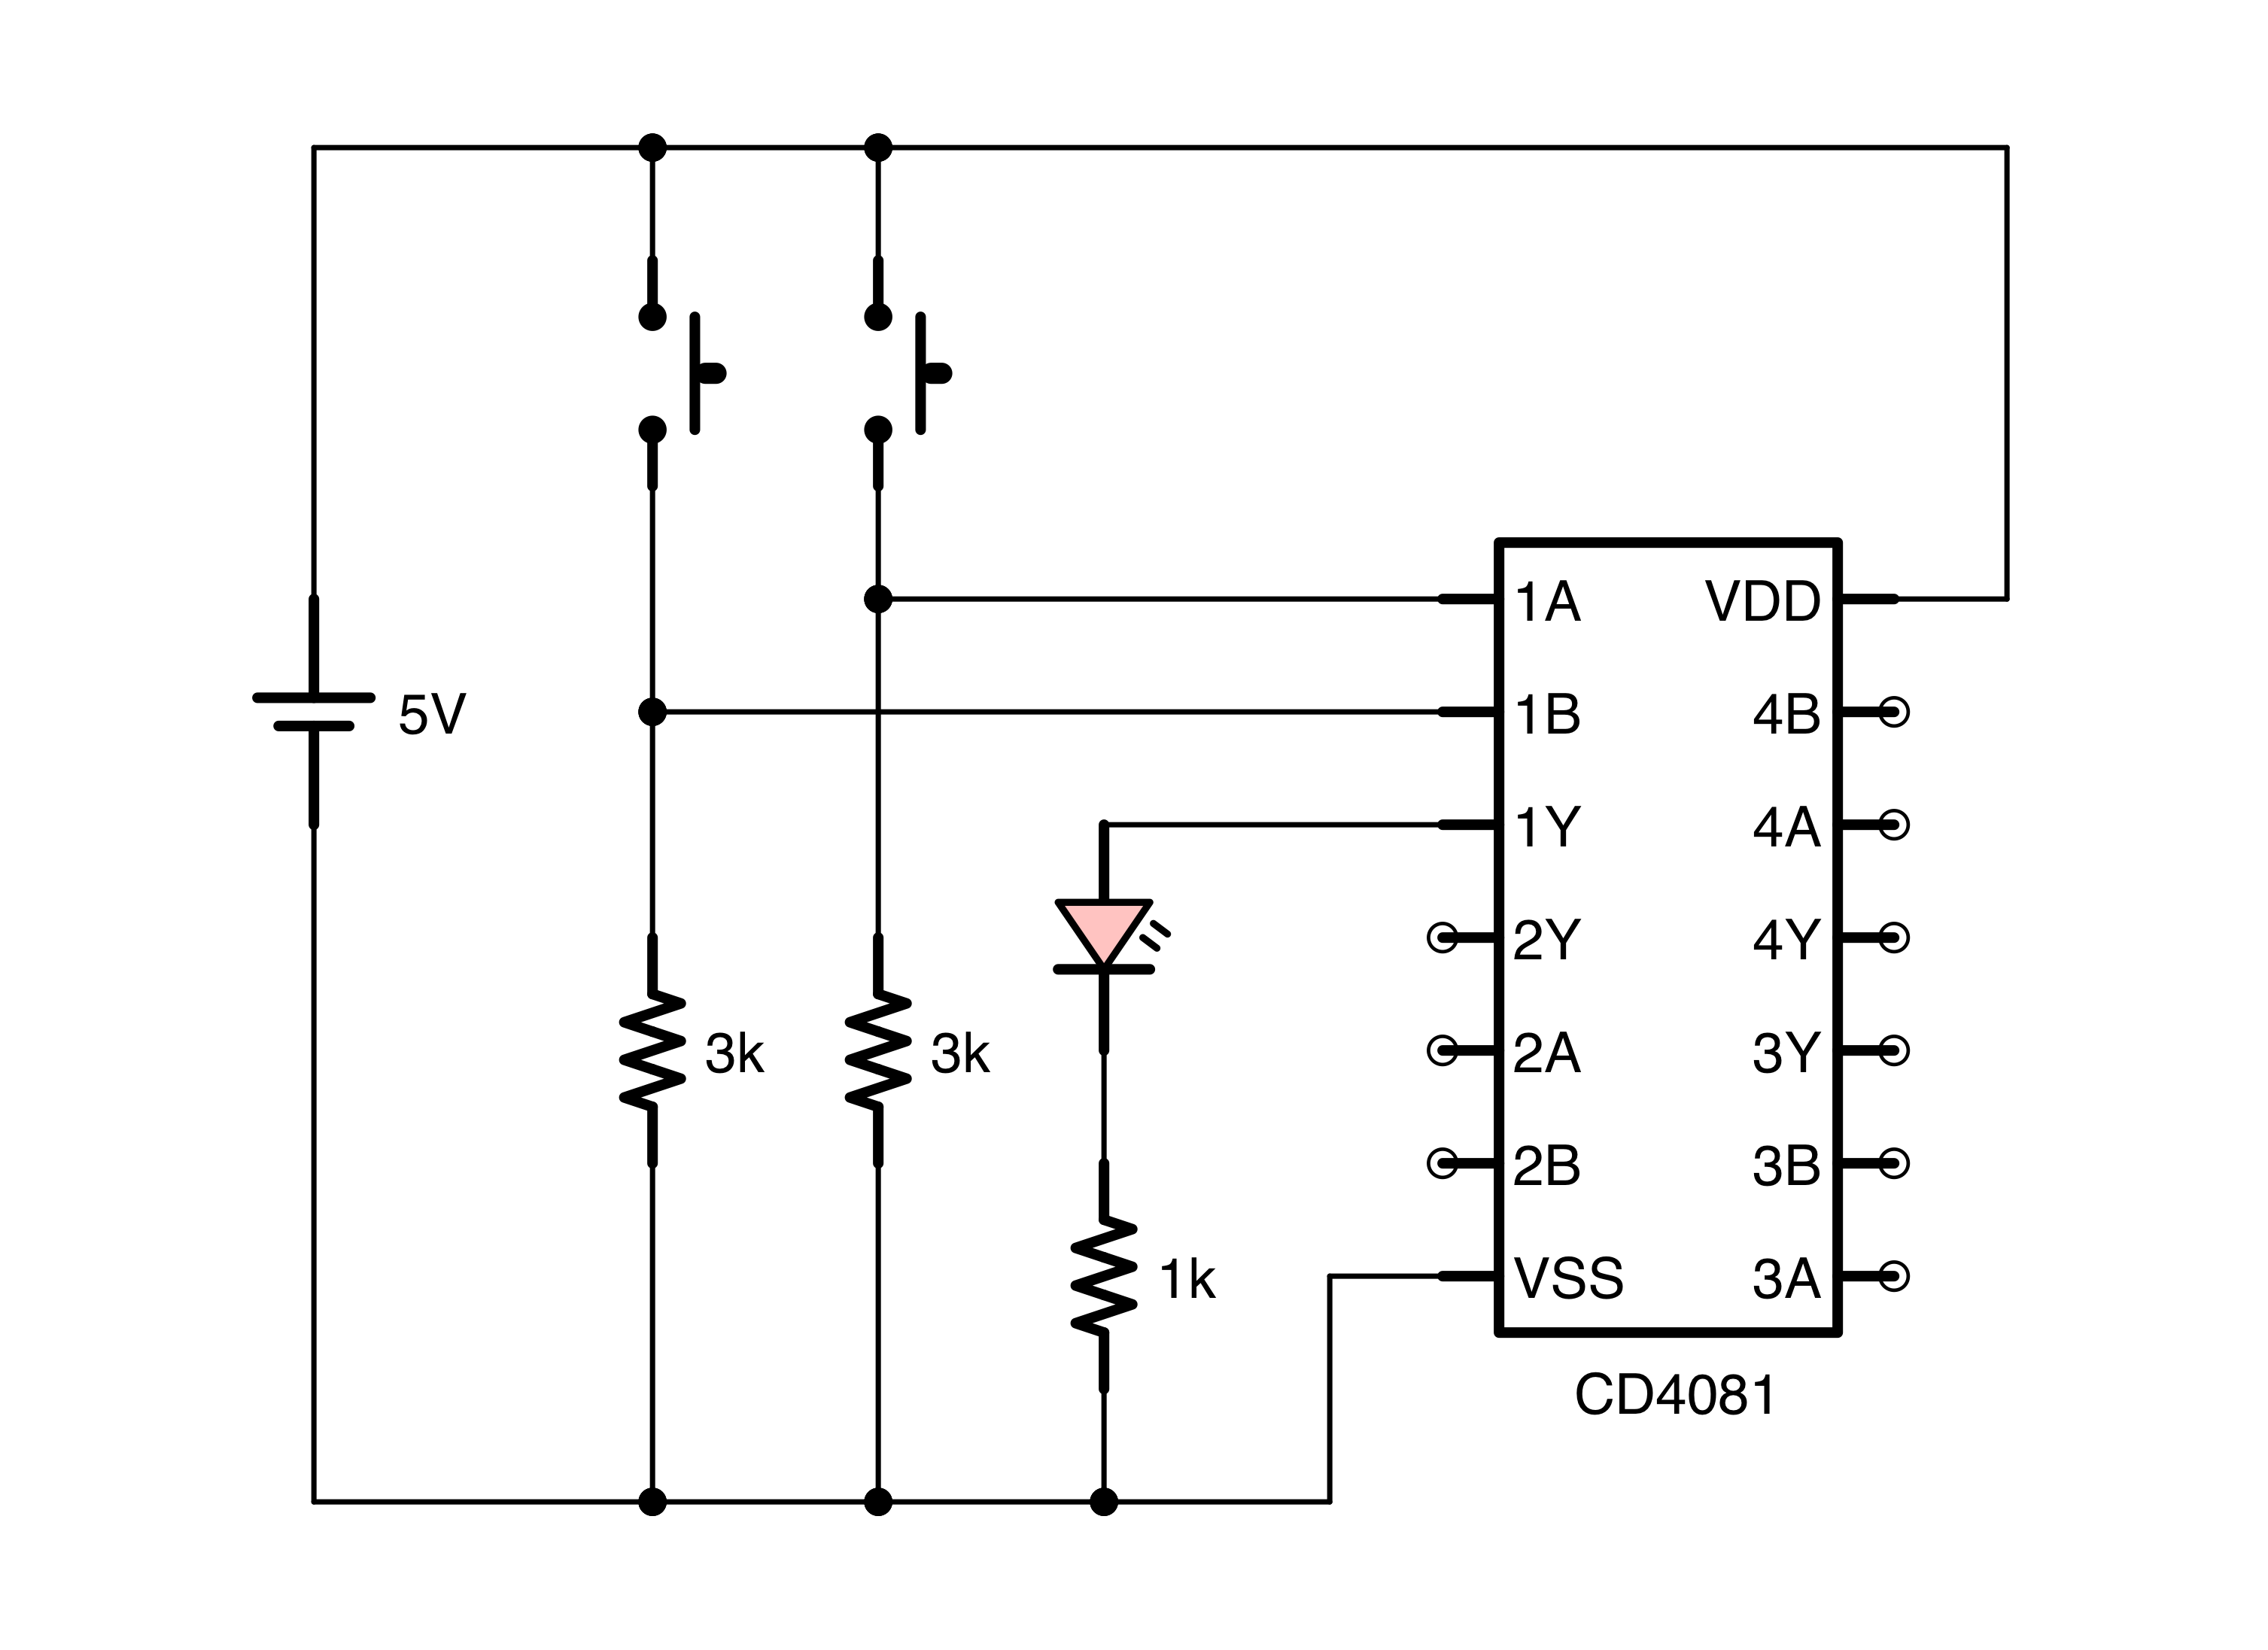
\includegraphics[width=\columnwidth]{LogicGateExample.png}

The 3k resistors are pull-down resistors.  The 1k resistor is a current-limiting resistor for the LED.
}
\item 
\question{Build the circuit in Figure~\ref{figLogicGateExample} (don't forget that the power source should be $5\myvolt$).}
\solution{When built, the circuit should only light up the LED when \emph{both} the buttons are pushed down.}
\item 
\question{If you assume that a negligible amount of current flows through the inputs of the AND gate, and that the output functions as a $5\myvolt$ voltage source (and the LED is red), how much current flows through each resistor when all of the buttons are pressed?  What, then, is the total current used by the circuit if you ignore the logic gate?}
\solution{The pull-down resistors each have $1.67\myamp$ of current, and the current-limiting resistor has $3.2\mymamp$ of current.  Therefore, the total current is $6.54\mymamp$.}
\explanation{When a button is pressed, there is a $3,000\myohm$ pull-down resistor connecting the power to ground.
Therefore, we can use Ohm's Law to find the current usage:
\begin{align*} 
I &= V / R \\
  &= 5 / 3,000 \\
  &= 0.00167\myamp = 1.67\mymamp
\end{align*}
Therefore, \emph{each} of the button circuits are using this amount of current.

Then, when both the inputs are positive, the output goes to $5\myvolt$.
This is dropped $1.8\myvolt$ by the red LED, leaving $3.2\myvolt$ for the resistor.
Therefore, the current going through the resistor is:
\begin{align*}
I &= V / R \\
  &= 3.2 / 1,000 \\
  &= 0.0032\myamp = 3.2\mymamp
\end{align*}
Therefore, the total amount of current in this circuit is $1.67 + 1.67 + 3.2 = 6.54\mymamp$.
}
\item 
\question{Measure the actual current that flows through each resistor.  If you are having trouble pushing the buttons while you measure the current, just replace the buttons with wires for this test.}
\solution{Your currents should roughly match the answers to the previous question.}
\item 
\question{Measure the current that it used by the AND gate itself.  You can do this by measuring the supply current of the AND gate.  Measure it both when its output is true and false.}
\solution{This measurement will vary depending on the brand of AND gate you are using.  However, usually it is less than $1\mymamp$ when the output is off.  It should increase by about the output current ($3.2\mymamp$) when the output is on.}
% FIXME - stopped adding solutions here.
\item 
\question{Draw a schematic of a circuit that has two buttons (B1 and B2) which light up an LED if either button is pressed.  Use the logic gate shapes for the schematic.}
\item 
\question{Draw a schematic of a circuit that has two buttons (B1 and B2) which light up an LED if neither button is pressed.  Use the logic gate shapes for the schematic.}
\item 
\question{Draw a schematic of a circuit that has four buttons (B1--B4) which light up an LED if either B1 and B2 are pressed or if B3 and B4 are pressed.  Use the logic gate shapes for the schematic.}
\item 
\question{Look at the construction of the different gates from NAND gates in Figure~\ref{figNANDLogic}.  Copy down the OR gate construction four times, and trace how the output is generated for each possible set of inputs (true/true, true/false, false/true, false/false).  Show the inputs and outputs on each NAND gate.  Compare the outputs to the truth table for the OR function in Figure~\ref{figTruthTable}.}
\item 
\question{Take the circuit in Figure~\ref{figLogicGateExample} and draw a schematic to use pull-up resistors on the inputs rather than pull-down resistors.  How will this change the behavior of the circuit?}
\item 
\question{Let's say that we want to create a door buzzer so that someone outside a door can push a button to be let in.  However, the person inside also wants a switch to be able to disable the buzzer.  The buzzer can be thought of as a simple device that buzzes when any positive voltage is applied.  Draw a circuit diagram of this setup using logic gates.  The buzzer can be drawn as a resistor labelled ``buzzer'' (don't forget to connect the other side to ground!).}
\end{enumerate}
